% !TeX root = statnicaEKT.tex
% !TeX spellcheck = cs_CZ
\part{BPC-ESI - Modelování a simulace obvodů}
{\huge Otázky:}
\newline
\begin{enumerate}
	\item Otázka - Princip simulace obvodů ve stejnosměrné, střídavé a časové oblasti. Modelování a analýza šumu v elektronických obvodech.
	\item Otázka - Toleranční a citlivostní analýza. Metody pro analýzu stability.
	\item Otázka - Modelování elektronických prvků, metody identifikace parametrů. Formální modely komplexních soustav. Využití analogií (elektro-tepelná, elektro-mechanická).
\end{enumerate}
\newpage
\chapter{První otázka}
\section{Princip simulace obvodů ve stejnosměrné oblasti DC}
Stejnosměrná analýza slouží k určení \textit{pracovního bodu} obvodu, tedy stejnosměrných napětí a proudů v ustáleném stavu. 
	\begin{itemize}
	\item Při DC analýze se střídavé zdroje nahrazují jejich stejnosměrnými složkami, obvykle nulou
	\item Akumulační prvky, tedy kondenzátory a induktory, se pro DC analýzu vyřazují z činnosti.
	\begin{itemize}
		\item Cívku nahradíme zkratem (induktor brání rychlým změnám amplitudy proudu, ale při vypuštění AC prvků je proud konstantní DC; v ideálním případě se chová jako vodič - zkrat)
		\item Kondenzátor vypustíme (kondenzátor se přirozeně nabije a poté přes něj již nemůže téct další DC proud; v ideálním případě se chová jako přerušený obvod)
		\item Po odstranění setrvačných prvků zmizí z obvodových rovnic čas.
		\textbf{Standardní stejnosměrná analýza proto nemůže poskytnout informaci o stabilitě či
		nestabilitě pracovního bodu.} (Aby bylo možné měření provést, musí být u
		reálného systému pracovní bod stabilní)
		\begin{figure}[H]
			\centering
			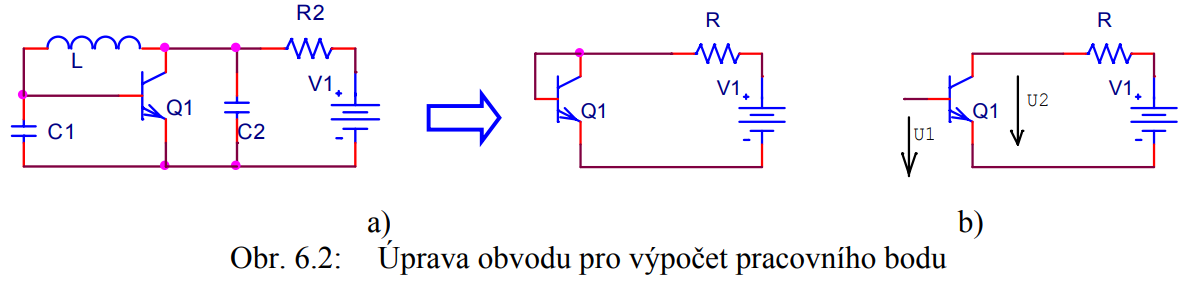
\includegraphics[width=0.6\linewidth]{Obrazky/ESI/simulaceDC}
			\caption{Úprava obvodu pro výpočet pracovního bodu}
			\label{fig:simulacedc}
		\end{figure}
	\end{itemize}
	\item Na cívce (při DC analýze) ideálně již není žádný úbytek napětí (nulový R i U), vypustí se její vliv v tomto případě také (obr. 6.2b vyjdřuje tedy zesilovač se společným emitorem SE)
	\item Pracovní bod se nachází tam, kde $U_1$ (vstup T - B-E) = $U_2$ (výstup T - C-E) $\rightarrow$ v pracovním bodě musí platit $U_1$ - $U_2$ = 0, to znázorňuje graf b)
		\begin{figure}[H]
			\centering
			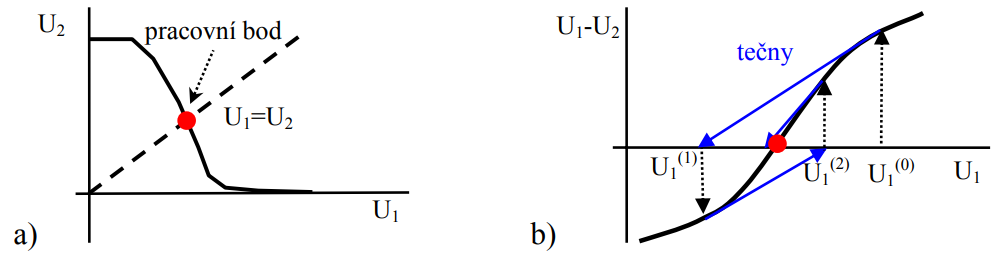
\includegraphics[width=0.55\linewidth]{Obrazky/ESI/simulaceDCpracBod}
			\caption{Princip výpočtu pracovního bodu}
			\label{fig:simulacedcpracbod}
		\end{figure}
	\item Při výpočtu pracovního bodu se používá Newton-Raphsonova metoda tečen
	\begin{itemize}
		\item Na počátku se zvolí bod $U_0^{(1)}$, pak $U_0^{(2)}$
		\item Výpočet probíhá iteračně dokud se nenajde průsečík na ose \textit{x} s dostatečně malou chybou
	\end{itemize}
	\item Konvergence není zaručena
	\begin{itemize}
		\item Problémy u obvodů s velkým ziskem, ostrými hranami, nelinearitou
		\item Výpočet probíhá iteračně dokud se nenajde průsečík na ose \textit{x} s dostatečně malou chybou
	\end{itemize}
\end{itemize}

\section{Princip simulace obvodů v střídavé oblasti AC}
Měří \textbf{kmitočtové charakteristiky} obvodu pracujícího v lineárním režimu.\\
Vstupní i výstupní veličiny mají harmonický průběh stejné frekvence a liší se jen amplitudou a fází (výsledkem: amplitudová a fázová charakteristika)\\ Nejprve se určí stejnosměrný pracovní bod a kolem něj se obvod zlinearizuje. Tím vznikne lineární model, který se řeší pro jednotlivé kmitočty.
\begin{figure}[H]
	\centering
	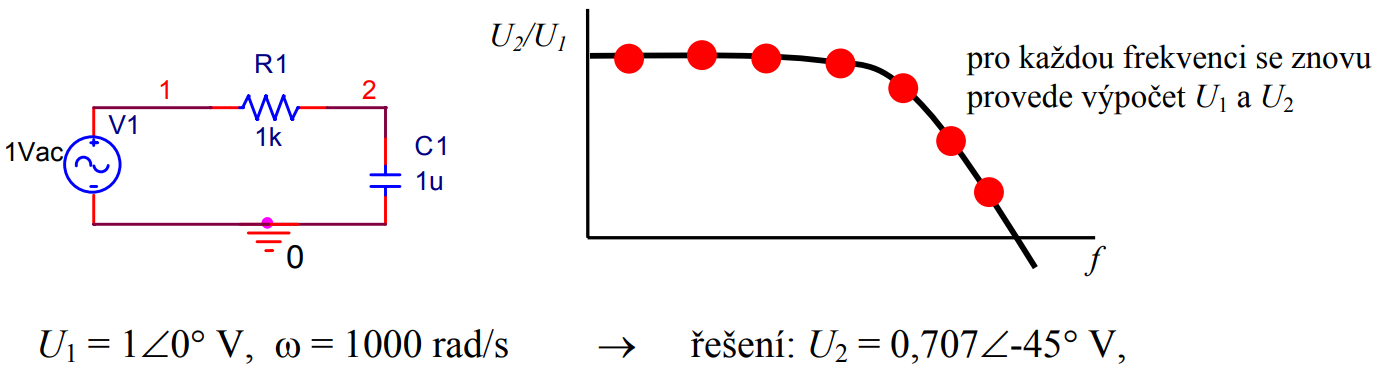
\includegraphics[width=0.55\linewidth]{Obrazky/ESI/simulaceAC}
	\caption{Výpočet střídavé odezvy integračního článku}
	\label{fig:simulaceac}
\end{figure}
\begin{itemize}
	\item \textbf{Řešení v harmonickém ustáleném stavu:}
	\begin{itemize}
		\item \underline{fázorovou metodou:} každá veličina je charakterizována komplexním číslem (nesoucí info o amplitudě i fázi příslušného čas. průběhu)
		\begin{itemize}
			\item kromě lineárních obvodů je fáz. analýzu možné použít i u obvodů s \textbf{nelinearitou jako parazitní vlastností} (filtry , zesilovače) - řešení linearizací v pracovním bodě $\rightarrow$ nahrazení charakteristiky tečnou v pracovním bodě (energie vyšších harmonických je zanedbatelná a obvod je charakterizován jen amplitudou a fází 1. harmonické)
		\end{itemize}
	\end{itemize}
	\item \textbf{Řešení při výrazné nelinearitě:}
	\begin{itemize}
		\item Výsledky střídavé analýzy jsou platné jen pro obvody pracující v lineárním režimu. Pro silně nelineární obvody výpočet sice proběhne, ale výsledky jsou neplatné.
		\begin{figure}[H]
			\centering
			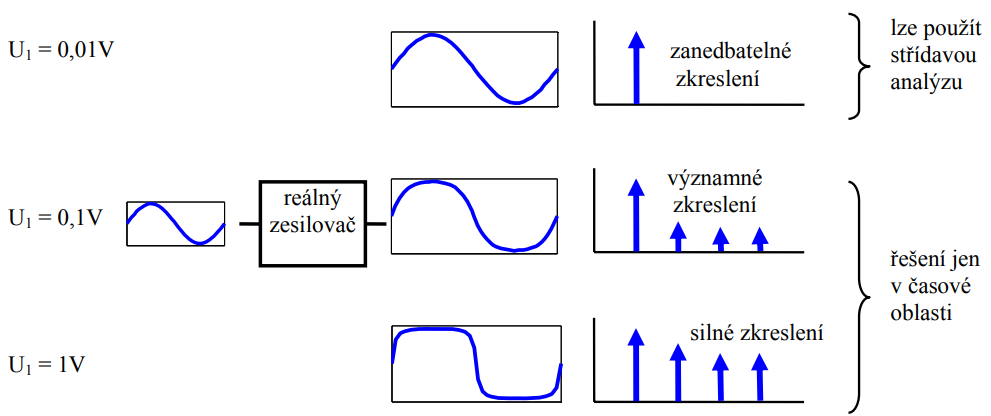
\includegraphics[width=0.5\linewidth]{Obrazky/ESI/simulaceACnelinearni}
			\caption{Střídavá analýza reálného zesilovače}
			\label{fig:simulaceacnelinearni}
		\end{figure}
		\item Obr.: Je-li amplituda vstupního napětí malá, tak že je na výstupu opět přibližně harmonický signál, výsledky střídavé analýzy se dobře shodují s realitou. Při zvyšování amplitudy na vstupu se začne uplatňovat nelinearita. Výstupní "sinusovka" začne být významně "deformovaná", tj. signál bude obsahovat vyšší složky spektra. Střídavá analýza již není použitelná, protože není splněn základní předpoklad, že všechna napětí a proudy jsou harmonické funkce.
		\item Příklady nelineárních obvodů: oscilátory, směšovače
	\end{itemize}
	\item Příklady využití: analýza zesilovačů, filtrů
\end{itemize}

\section{Princip simulace obvodů v časové oblasti}
Měření pomocí signálového generátoru na vstupu vedení; měří se osciloskopem.\\
Výsledkem analýzy: časové průběhy napětí $u(t)$ a proudu $i(t)$ navzorkované v časech $t$
\begin{figure}[H]
	\centering
	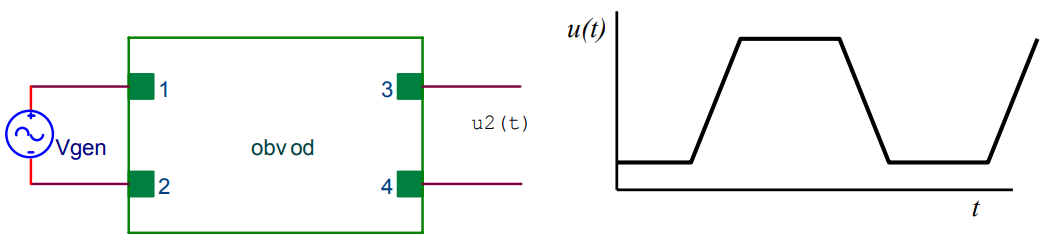
\includegraphics[width=0.5\linewidth]{Obrazky/ESI/simulaceCAS}
	\caption{Výsledky časové analýzy}
	\label{fig:simulacecas}
\end{figure}

\begin{itemize}
	\item Simulátor postupuje po časových krocích a v každém kroku numericky řeší stav obvodu
	\begin{itemize}
		\item Výsledek ukazuje přechodné děje i ustálený stav
		\item Délka kroku se nastavuje dynamicky podle aktuální strmosti (v případě malých změn se volí krok větší, při strmé nástupné hraně se krok zkracuje) a požadované přesnosti
		\item Pokud se mezi kroky objeví strmá nástupní hrana, v čase $t_3$ vznikne velká chyba a výsledek se zamítne. Program se vrátí do $t_2$ a pokračuje s menším krokem. Proces zkracování probíhá tak dlouho, dokud se nedosáhne akceptovatelné chyby. Pokud je chyba naopak příliš malá, krok se prodlužuje.
		\begin{figure}[H]
			\centering
			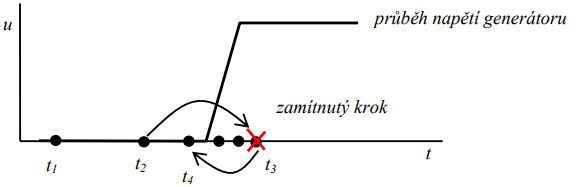
\includegraphics[width=0.5\linewidth]{Obrazky/ESI/simulaceCASkroky}
			\caption{Princip automatické volby časového kroku}
			\label{fig:simulacecaskroky}
		\end{figure}
		
	\end{itemize}
	\item Není-li možné dodržení předepsané chyby $\rightarrow$ změny v obvodu/analýze:
	\begin{itemize}
		\item použití spojitých a hladkých funkcí (doplněním o parazitní \textbf{kapacitu} - krátký delay než se kondenzátor nabije; doplněním o parazitní \textbf{indukčnost} - cívká brání okamžitým skokům)
		\item nepoužívání ideálních impulzních signálů (s 0 délkou hrany)
	\end{itemize}
	\item Metoda je stabilní tehdy, pokud se malé chyby vzniklé aproximací nebo zaokrouhlením v dalších krocích nezesilují.
	\begin{itemize}
		\item \underline{Lichoběžníková metoda:} výpočet jako průměr sklonu na začátkua a na konci kroku; může dělat umělé kmity
		\item \underline{Gearova metoda:} výpočet z více předchozích časových kroků, ne jen z posledního; tlumenější a potlačuje numerické kmity
	\end{itemize}
	\item Volba počátečních podmínek (pracovního bodu):
	\begin{itemize}
		\item \textbf{ze stejnosměrného pracovního bodu obvodu} - nejprve se vypočítá ustálený stav před začátkem děje a z něj se převezme počáteční napětí kondenzátorů a proud cívek
		\item \textbf{přímé nastavení počátečního bodu} - při simulaci např. zapnutí obvodu z nenabitého stavu, vybíjení kondenzátoru (= děj, co neodpovídá předem ustanovenému pracovnímu bodu)
	\end{itemize}
	\item Příklady využití: analýza spínaných obvodů (ostré hrany), nabíjení a vybíjení kondenzátorů, dynamické děje v zesilovačích
\end{itemize}
\section{Shrnutí rozdílů}
Pro DC analýzu hledáme pracovní bod, pro AC analýzu zkoumáme malé signály kolem pracovního bodu a pro transient analýzu sledujeme skutečný průběh veličin v čase. Rozdíl je hlavně v tom, jaký model obvodu se použije a které prvky se při výpočtu berou v úvahu.

\section{Modelování a analýza šumu v elektronických obvodech}
\subsection{Šum}
Nežádoucí náhodné napětí nebo proud, který se přidává k užitečnému signálu. V elektronických obvodech vzniká například v rezistorech (tepelný šum - bílý), polovodičových součástkách nebo v aktivních prvcích. Šum omezuje citlivost zesilovačů, kvalitu měření i přenos dat.\\
Šum obecně popisujeme \textbf{spektrální hustotou výkonu} $G(f)$ [$W/Hz$]
\subsection{Modelování šumu}
Pro analýzu šumu se při teoretickém modelování obvodu skutečné součástky nahrazují modely, které kromě ideálního chování obsahují i šumové zdroje. Tyto zdroje se přidávají do modelu tak, aby vystihly fyzikální zdroj šumu dané součástky. Smyslem modelování je určit, jak se šum jednotlivých prvků promítne na výstup obvodu.\\
Modely:
\begin{itemize}
	\item Rezistor - modeluje se šumovým napěťovým nebo proudovým zdrojem (sami vytvářejí teplo)
	\item Dioda a tranzistor - kombinací proudových zdrojů
	\item Operační zesilovač - vstupním napěťovým šumem a vstupním proudovým šumem (popisují jeho reálné rušení na vstupech)
\end{itemize}
\subsection{Princip analýzy šumu} 
- Metoda aplikovatelná jen pro lineární obvody \textit{(stejně jako AC)}\\
Šumová analýza vychází z linearizovaného obvodu v pracovním bodě. Zkoumá se přenos šumových zdrojů od jejich vzniku až na sledovaný výstup. Výsledkem bývá spektrální hustota šumového napětí nebo proudu, případně celkové efektivní šumové napětí v zadaném pásmu.\\
Obvyklý postup je tento:
\begin{enumerate}
	\item Určí se stejnosměrný pracovní bod obvodu.
	\item Obvod se zlinearizuje.
	\item Uvažují se ekvivalentní šumové zdroje jednotlivých součástek.
	\item Určí se šumový příspěvek na výstupu.
	\item Výsledky se vyhodnotí v daném kmitočtovém pásmu.
\end{enumerate}
Filtry pro potlačení šumu:
\begin{enumerate}
	\item Dolní propust
	\item Horní propust
	\item Pásmová propust
	\item Pásmová zdrž (vyřízne konkrétní rušivou frekvenci)
	\item Pasivní filtry: RC, LC (kombinace rezistoru/tlumivky a kondenzátoru)
	\begin{itemize}
		\item \textbf{RC filtr} - Rezistor omezí proud a kondenzátor propouští rychlé změny do země (rušivé krátké špičky a vysokofrekvenční složky se přes něj odvedou pryč místo toho, aby pokračovaly dál do obvodu.)
		\item \textbf{LC filtr} - Tlumivka brání rychlým změnám proudu velkou impedancí (potlačení vysokofrekvenčního rušení a proudových špiček)
		\item \textbf{$\Pi$ filtr $\rightarrow$ \textit{C-L-C}} - 1. \textit{C} zachytí vysokofrekvenční rušení a odvede ho do země. Tlumivka \textit{L} pak brání průchodu rychlých změn proudu a 2. \textit{C} zbylé rušení opět uzemní.
	\end{itemize}
\end{enumerate}

\subsection{Význam šumové analýzy}
U zesilovačů malých signálů, senzorových obvodů, měřicích přístrojů a komunikačních systémů. Pomáhá určit, která součástka nebo blok je hlavním zdrojem rušení a jak lze šum zmenšit.

\newpage
\chapter{Druhá otázka}

\section{Základní pojmy -- toleranční analýza a syntéza}
Nedílnou fází každého návrhového postupu je analýza chování obvodu nejen při jmenovitých hodnotách parametrů, ale i při odchylkách od těchto hodnot.
\begin{itemize}
    \item \textbf{Toleranční analýza} -- na základě znalosti odchylek \textbf{parametrů prvků} určujeme odchylku nějaké \textbf{charakteristické vlastnosti} obvodu (zesílení, délky hran, oscilační frekvence).
    \item \textbf{Toleranční syntéza} -- opačná úloha: z maximálních povolených odchylek charakteristiky obvodu určujeme maximální tolerance prvků.
\end{itemize}
Parametry obvodových prvků tvoří $r$-rozměrný vektor $\boldsymbol{\alpha} = [\alpha_1, \ldots, \alpha_r]^T$ s nominálními hodnotami $\boldsymbol{\alpha}^{(0)}$. \textbf{Toleranční oblast} $R_T$ v prostoru parametrů je $r$-rozměrný kvádr daný $\alpha_{di} \le \alpha_i \le \alpha_{hi}$.
Charakteristické vlastnosti tvoří vektor $\mathbf{y} = [y_1, \ldots, y_n]^T$. \textbf{Přípustná oblast} $R_A$ v prostoru charakteristik je dána nerovnostmi $y_{dj} \le y_j \le y_{hj}$.\\
Nominálním hodnotám $\boldsymbol{\alpha}^{(0)}$ odpovídá \textbf{návrhový střed} $\mathbf{y}^{(0)}$.

\section{Praktické metody toleranční analýzy}
Pro větší systémy jsou dostupné tři základní metody:
\begin{enumerate}
    \item \textbf{Citlivostní analýza} -- předpokládá lineární závislost charakteristiky na parametrech; ze znalosti tolerancí přímo odhadne rozptyl sledované charakteristiky.
    \item \textbf{Analýza nejhoršího případu (Worst Case)} -- stanoví nejhorší možnou kombinaci hodnot prvků, kdy dojde k největší odchylce sledované charakteristiky od nominální hodnoty. Sledovaná charakteristika musí záviset monotónně na všech parametrech.
    \item \textbf{Analýza Monte Carlo} -- simulace hromadné výroby; pomocí generování náhodných odchylek parametrů určí statistické parametry sledované charakteristiky včetně výtěžnosti. Nemá žádné omezující podmínky, ale je výpočetně náročná.
\end{enumerate}

\section{Citlivostní analýza}
Uvažujeme závislost sledované charakteristiky obvodu $y$ na jednom obvodovém parametru $\alpha$. V malém okolí nominálních hodnot nahrazujeme křivku její tečnou. Směrnice tečny se nazývá \textbf{absolutní citlivost} $y$ na $\alpha$:
\[
    S_\alpha^y = \frac{dy}{d\alpha}
\]
Pro odchylku $\Delta y$ pak platí přibližně $\Delta y \approx S_\alpha^y \cdot \Delta\alpha$.

\begin{figure}[H]
    \centering
    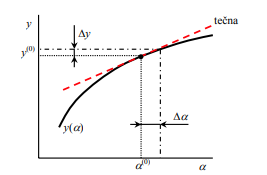
\includegraphics[width=0.55\linewidth]{Obrazky/ESI/citlivost}
    \caption{K definici citlivosti: křivka $y(\alpha)$ a tečna v nominálním bodě $\alpha^{(0)}$}
    \label{fig:citlivost}
\end{figure}

Absolutní citlivost neumožňuje srovnávat vliv různých prvků (mají různé jednotky). Proto se zavádí \textbf{relativní (normovaná) citlivost}:
\[
    S_{R\alpha}^y = \frac{\alpha^{(0)}}{y^{(0)}} \frac{dy}{d\alpha}
\]
Číselně udává, o kolik \% se změní sledovaná veličina, když se obvodový parametr změní o 1\%.\\
V PSpice se používá \textbf{semirelativní citlivost}: $S_{S\alpha}^y = \frac{\alpha^{(0)}}{100} \frac{dy}{d\alpha}$ -- udává absolutní změnu $y$, když se parametr změní o 1\%.

Při uvažování více parametrů se příspěvky sčítají: $\Delta y \approx \sum S_{\alpha_i}^y \Delta\alpha_i$.\\
\textbf{Nejhorší případ} (všechny odchylky stejného znaménka, na hranici tolerančního pásma $t_i$):
\[
    \left|\frac{\Delta y_{\max}}{y^{(0)}}\right| \approx \left|S_{R\alpha_1}^y\right| t_1 + \ldots + \left|S_{R\alpha_r}^y\right| t_r
\]
\textbf{Statistický případ} (nekorelované odchylky diskrétních prvků):
\[
    \left|\frac{\Delta y_{\max}}{y^{(0)}}\right|_{\text{stat}} \approx \sqrt{\left(S_{R\alpha_1}^y\, t_1\right)^2 + \ldots + \left(S_{R\alpha_r}^y\, t_r\right)^2}
\]
Statistický případ dává realističtější (méně pesimistický) odhad než nejhorší případ.

\section{Analýza nejhoršího možného případu -- Worst Case}
Hledá takovou kombinaci parametrů prvků v rámci tolerančního pásma, kdy se sledovaná charakteristika nejvíce odchýlí od jmenovité hodnoty. Pokud taková hodnota leží v $R_A$, lze očekávat 100\% výtěžnost.

Při malých odchylkách (platnost lineární aproximace) je nejhorší případ vždy dán \textbf{krajními hodnotami} parametrů. Ze znamének citlivostí v nominálních hodnotách parametrů se určí, která ze dvou krajních hodnot znamená nejhorší případ -- stačí tedy jen $r$ výpočtů (pro $r$ parametrů).

\begin{figure}[H]
    \centering
    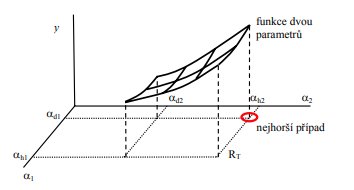
\includegraphics[width=0.60\linewidth]{Obrazky/ESI/worstcase}
    \caption{Princip analýzy Worst-Case: nejhorší případ leží v rohu toleranční oblasti $R_T$}
    \label{fig:worstcase}
\end{figure}

\section{Analýza Monte Carlo}
Metoda spočívá v mnohokrát opakované analýze uvažované soustavy s parametry součástek náhodně generovanými ve shodě s jejich skutečnými statistickými vlastnostmi -- simulace hromadné výroby. Nemá žádná omezení, na rozdíl od citlivostní analýzy postihuje i nelineární chování, ale je výpočetně náročná.

\subsection{Rozložení hustoty pravděpodobnosti}
Při výrobě součástek dochází k výrobnímu rozptylu -- parametry konkrétního prvku nejsou předem známé. Vykazují jistou náhodnost popsanou \textbf{hustotou pravděpodobnosti} $p(x)$:
\begin{itemize}
    \item \textbf{Rovnoměrné (Uniform)} rozdělení -- všechny hodnoty v tolerančním pásmu jsou stejně pravděpodobné; hodnota parametru prvku se nachází v intervalu $\text{NOM} \pm \text{TOL}$.
    \item \textbf{Normální (Gaussovo)} rozdělení -- hodnoty v blízkosti nominální hodnoty jsou pravděpodobnější; tolerance se uvažuje jako $1\sigma$. V praxi se generování omezuje na $\pm 3\sigma$.
\end{itemize}
Klíčové vlastnosti normálního rozdělení: $\pm\sigma$ pokrývá 68,3\%; $\pm 2\sigma$ pokrývá 95,5\%; $\pm 3\sigma$ pokrývá 99,7\% hodnot.

\begin{figure}[H]
    \centering
    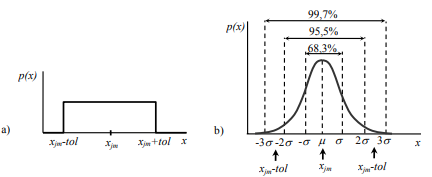
\includegraphics[width=0.70\linewidth]{Obrazky/ESI/rozdeleni}
    \caption{Rovnoměrné (vlevo) a normální/Gaussovo (vpravo) rozdělení hustoty pravděpodobnosti}
    \label{fig:rozdeleni}
\end{figure}

\subsection{Výtěžnost a histogram}
Výsledkem Monte Carlo analýzy je statistické rozdělení sledované charakteristické vlastnosti obvodu -- zobrazené jako \textbf{histogram}. \textbf{Výtěžnost} (yield) je pravděpodobnost, že soustava realizovaná ze součástí s hodnotami v tolerančních mezích bude vyhovující (sledované charakteristiky leží v $R_A$).

\begin{figure}[H]
    \centering
    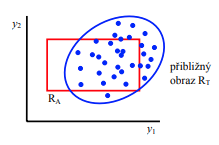
\includegraphics[width=0.65\linewidth]{Obrazky/ESI/montecarlo}
    \caption{Výsledky analýzy Monte Carlo: histogram mezní frekvence dolní propusti ze 500 běhů simulace (PSpice)}
    \label{fig:montecarlo}
\end{figure}

Pod histogramem PSpice zobrazuje: \texttt{mean} (střední hodnota), \texttt{sigma} (směrodatná odchylka), \texttt{minimum}/\texttt{maximum}, \texttt{median} a kvantily (10th, 90th \%ile).

\section{Metody pro analýzu stability}
Systém je stabilní, pokud všechny omezené vstupní signály vyvolají omezenou odezvu na výstupu. Prakticky: přechodná složka na výstupu s časem zaniká. Stabilita se zkoumá pomocí malosignálového (linearizovaného) modelu systému.

\subsection{Kořeny charakteristické rovnice -- póly přenosové funkce}
\textit{Systém je stabilní, pokud všechny kořeny charakteristické rovnice, resp. všechny póly přenosové funkce mají zápornou reálnou část.}
\begin{itemize}
    \item Pól s zápornou reálnou částí $\rightarrow$ přechodný děj s časem zaniká.
    \item Pól na imaginární ose $\rightarrow$ trvalé neustupující kmity (hraniční případ).
    \item Pól s kladnou reálnou částí $\rightarrow$ nestabilita, narůstající kmity.
\end{itemize}
Problémem je, že rozložení kořenů nelze přímo měřit a ani při počítačové simulaci nelze toto rozložení stoprocentně spolehlivě určit (iterační algoritmy, konečná přesnost čísel).

\subsection{Nyquistovo kriterium}
Umožňuje zjistit stabilitu zpětnovazební soustavy pouze na základě frekvenční charakteristiky přenosu otevřené smyčky $B(j\omega)A(j\omega)$. Je vhodné jak pro počítačovou simulaci, tak pro praktické měření.\\
\textit{Systém je stabilní tehdy a jen tehdy, když:}
\begin{enumerate}
    \item \textit{je stabilní jeho rozpojená zpětnovazební smyčka,}
    \item \textit{frekvenční charakteristika $B(j\omega)A(j\omega)$ v komplexní rovině neobepíná kritický bod $(1, j0)$ ani jím neprochází.}
\end{enumerate}

\begin{figure}[H]
    \centering
    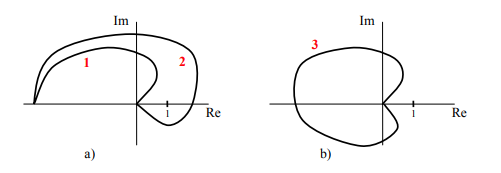
\includegraphics[width=0.65\linewidth]{Obrazky/ESI/nuqists}
    \caption{Nyquistovy charakteristiky: a) stejnosměrný zesilovač -- křivka 1 stabilní, křivka 2 nestabilní; b) střídavý zesilovač}
    \label{fig:nyquist}
\end{figure}

\subsection{Bodeho metoda -- fázová jistota a jistota zisku}
Praktičtější alternativa k Nyquistovu diagramu. Hodnotí se přenos otevřené smyčky $BA(j\omega)$ v Bodeho frekvenčních charakteristikách (modul v dB a fáze):
\begin{itemize}
    \item \textbf{Fázová jistota PM} (Phase Margin) -- úhel zjištěný při kmitočtu, kde modul $|BA| = 1$ (tj. 0\,dB). Pokud je tento úhel nulový nebo záporný $\rightarrow$ zesilovač po uzavření zpětnovazební smyčky kmitá.
    \item \textbf{Jistota zisku GM} (Gain Margin) -- modul $|BA|$ zjištěný při kmitočtu, kde fázový posun je nulový. Tento modul musí být menší než 1 (záporný v dB). Není-li podmínka splněna $\rightarrow$ zesilovač kmitá.
\end{itemize}
\textbf{Bodeho doporučení:} PM $\geq 60°$ a GM $\geq 10$\,dB pro spolehlivou stabilitu. (Hodnota PM ovlivňuje překmit přechodové odezvy -- pro PM = 45°: překmit 23\%, PM = 60°: překmit 9\%.)

\begin{figure}[H]
    \centering
    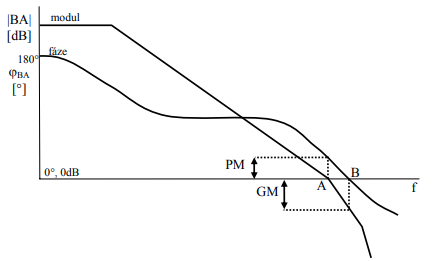
\includegraphics[width=0.70\linewidth]{Obrazky/ESI/bodeho}
    \caption{Bodeho charakteristiky otevřené smyčky a postup zjištění fázové jistoty PM a jistoty zisku GM}
    \label{fig:bode}
\end{figure}

\subsection{Kompenzace}
Pokud navržený obvod nedosahuje požadovaných PM a GM, použije se \textbf{kompenzace} -- dodatečná úprava frekvenční charakteristiky přenosu $BA$:
\begin{itemize}
    \item \textbf{Integrační kompenzace} -- přidání dalšího pólu na nízkou frekvenci (RC článek). Posouvá charakteristiku tak, aby první lom nastal na ose 0\,dB a zajistil PM $\geq 45°$. Nevýhoda: snížení šířky přenášeného pásma.
    \item \textbf{Integračně-derivační kompenzace} -- přidání pólu i nuly (RC článek R1+R2, C). Frekvence nuly kompenzuje původně první lom, čímž lze dosáhnout PM $\geq 45°$ při vyšším kmitočtu průchodu nulou. Menší ztráta šířky pásma než u integrační kompenzace.
    \item \textbf{Derivační kompenzace} -- přidání nulového bodu k přenosové funkci (kompenzuje původní druhý lom). Snižuje zálohu zisku ZV systému; nevýhodou je pokles zisku na nízkých kmitočtech.
\end{itemize}

\newpage
\chapter{Třetí otázka}

\section{Modelování elektronických prvků}
\textit{Modelem fyzikálního objektu nazýváme reprezentaci tohoto objektu symbolickým popisem (rovnicemi) nebo jiným objektem (náhradní schéma), který z hlediska zkoumaných vlastností nahrazuje modelovaný objekt.}\\
Vzhledem k využití počítačů je modelem elektronického prvku vždy soustava rovnic -- \textbf{matematický model}. Na úrovni obvodové simulace tyto modely popisují vztahy mezi svorkovými veličinami (napětí a proudy). V rovnicích vystupují různé koeficienty -- \textbf{parametry modelu}.

\begin{figure}[H]
    \centering
    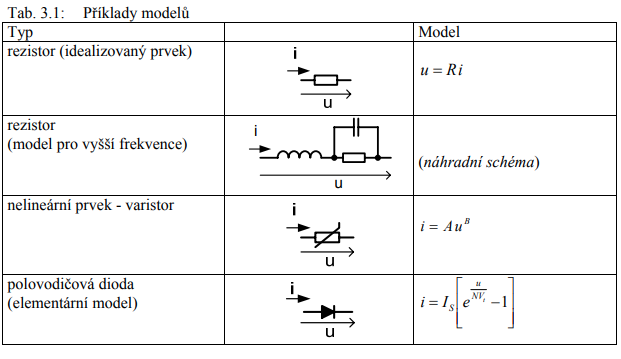
\includegraphics[width=0.70\linewidth]{Obrazky/ESI/models_tab}
    \caption{Příklady modelů elektronických prvků: rezistor (ideální i pro vyšší frekvence), varistor, polovodičová dioda (Tab. 3.1)}
    \label{fig:modely_tab}
\end{figure}

Matematický model celého obvodu vznikne sloučením modelů dílčích prvků s Kirchhoffovými rovnicemi, které popisují interakce mezi prvky. Jedná se o soustavu algebraicko-diferenciálních rovnic.

\subsection{Model bipolárního tranzistoru (BJT)}
Pro stejnosměrnou analýzu (nastavení pracovního bodu) stačí tři parametry: $U_{BE}$, proudový zesilovací činitel $\beta$ a zbytkový kolektorový proud $I_{CB0}$.

\begin{figure}[H]
    \centering
    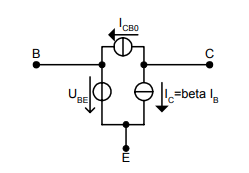
\includegraphics[width=0.40\linewidth]{Obrazky/ESI/bjt_trans}
    \caption{Model bipolárního tranzistoru pro návrh pracovního bodu (Obr. 10.16)}
    \label{fig:bjt_model}
\end{figure}

Malosignálové parametry jsou určené převážně kolektorovým proudem $I_C$. Pro analýzu v linearizovaném obvodu (AC oblast) se používá \textbf{Giacolettův fyzikální model}:
\begin{itemize}
    \item strmost: $g_m = \frac{1}{U_T} I_C \approx 35\,I_C$ (kde $U_T$ je teplotní napětí)
    \item výstupní odpor: $r_o = \frac{V_E}{I_C}$ ($V_E$ je Earlyho napětí, typicky 100\,V)
    \item vstupní odpor: $r_\pi = \frac{\beta}{g_m}$
    \item vstupní kapacita: $C_\pi \approx \frac{g_m}{2\pi f_T}$ ($f_T$ je tranzitní frekvence)
    \item průchozí kapacita $C_\mu$, výstupní kapacita $C_{CE}$
\end{itemize}

\subsection{Model unipolárního tranzistoru (FET)}
Pro nastavení pracovního bodu v saturační oblasti platí:
\[ I_D = K(U_{GS} - U_{TH})^2 \quad \text{pro } U_{GS} > U_{TH} \]
Malosignálové parametry: $g_m = 2\sqrt{K\,I_D}$, $r_o = \frac{1}{\lambda\,I_D}$.

\begin{figure}[H]
    \centering
    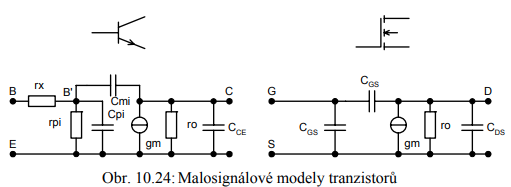
\includegraphics[width=0.7\linewidth]{Obrazky/ESI/malosig_model}
    \caption{Malosignálové modely tranzistorů: bipolární (vlevo) a unipolární (vpravo) -- Obr. 10.24}
    \label{fig:malosig_model}
\end{figure}

\section{Metody identifikace parametrů}
\textbf{Identifikací modelu} rozumíme postup pro získání jeho matematického popisu (rovnic). Velmi často se identifikací nazývá pouze proces získání parametrů, když je tvar rovnice předem znám.

\begin{itemize}
    \item \textbf{Z katalogového listu} -- výrobce uvádí typické a mezní hodnoty (např. $\beta$, $f_T$, $V_E$). Tyto hodnoty platí pro typický kus, skutečný prvek může mít odchylku v řádu desítek procent.
    \item \textbf{Z měření} -- změříme voltampérové nebo frekvenční charakteristiky konkrétního kusu a parametry modelu určíme proložením naměřených dat modelovou funkcí (curve fitting).
    \item \textbf{Numerická optimalizace} -- minimalizujeme odchylku mezi simulovanou a naměřenou charakteristikou jako účelovou funkci (kvadratická nebo maximální odchylka). Používají ji programy jako PSpice Model Editor.
    \item \textbf{Z fyzikální analýzy} -- parametry se odvodí z geometrie a technologie výroby součástky (vhodné pro integrované obvody).
\end{itemize}
\textbf{Důležité upozornění:} Kvalita modelů určuje věrohodnost výsledků simulací. Není možné přeceňovat výsledky simulací, pokud nemáme důkladně prověřeny modely. Navíc modely pro stejný typ součástky se liší kus od kusu (výrobní rozptyl).

\section{Formální modely komplexních soustav}
Soustavu se soustředěnými parametry lze plně popsat souborem prvků a definicí vzájemného propojení jejich uzlů -- \textbf{netlistem}. Tento formální popis je základem simulačních programů třídy Spice.

\begin{itemize}
    \item \textbf{Netlist} -- textový seznam prvků a jejich propojení (uzlů). Např.:
    \begin{center}
    \texttt{R1 1 2 1k} \quad \texttt{C1 2 0 1n} \quad \texttt{Q1 3 2 0 BC546A}
    \end{center}
    \item \textbf{Hierarchické modely (podvobvody, subcircuits)} -- složitý blok (např. operační zesilovač) se popisuje jako podvobvod s vnějšími svorkami. Uvnitř může být libovolně složitá síť prvků.
    \item \textbf{Makromodely} -- zjednodušené náhradní schéma komplexního bloku, které vystihuje jeho chování na svorkovém úrovni (vstup/výstup), ale ne vnitřní fyzikální strukturu. Jsou výpočetně méně náročné.
    \item \textbf{Stavový popis} -- soustava diferenciálních rovnic $\dot{\mathbf{x}} = A\mathbf{x} + B\mathbf{u}$, $\mathbf{y} = C\mathbf{x} + D\mathbf{u}$. Používá se pro systémovou analýzu (přenosové funkce, stabilita).
\end{itemize}

\section{Využití analogií}
Různé fyzikální systémy mohou být popsány matematicky shodnými rovnicemi. Tato \textbf{analogie} umožňuje použít obvodový simulátor (Spice) k simulaci tepelných nebo mechanických soustav.

\subsection{Elektro-tepelná analogie}
Přenos tepla je řízen rovnicemi formálně shodnými s Ohmovým zákonem a Kirchhoffovými zákony:

\begin{center}
\begin{tabular}{lll}
\toprule
\textbf{Elektrická veličina} & \textbf{Tepelná veličina} & \textbf{Jednotka} \\
\midrule
Napětí $U$ & Teplota (rozdíl) $\Delta T$ & K \\
Proud $I$ & Tepelný tok (výkon) $P$ & W \\
Odpor $R$ & Tepelný odpor $R_{th}$ & K/W \\
Kapacita $C$ & Tepelná kapacita $C_{th}$ & J/K \\
\bottomrule
\end{tabular}
\end{center}

Základní vztah: $\Delta T = R_{th} \cdot P$ (analogicky $U = R \cdot I$).\\
Tepelná kapacita modeluje akumulaci tepla: $P = C_{th} \frac{d(\Delta T)}{dt}$ (analogicky $i = C \frac{du}{dt}$).\\
Příklad použití: simulace oteplení výkonového tranzistoru -- model pouzdra (junction-case-ambient) jako RC řetězec.

\subsection{Elektro-mechanická analogie}
Mechanická soustava s hmotou, pružinou a tlumičem se chová analogicky k elektrickému LC obvodu:

\begin{center}
\begin{tabular}{lll}
\toprule
\textbf{Elektrická veličina} & \textbf{Mechanická veličina} & \textbf{Jednotka} \\
\midrule
Napětí $U$ & Síla $F$ & N \\
Proud $I$ & Rychlost $v$ & m/s \\
Indukčnost $L$ & Hmotnost $m$ & kg \\
Kapacita $C$ & Poddajnost $1/k$ & m/N \\
Odpor $R$ & Mechanický odpor $b$ (tlumení) & N$\cdot$s/m \\
\bottomrule
\end{tabular}
\end{center}

Newtonův zákon $F = m\ddot{x} + b\dot{x} + kx$ je analogický k rovnici RLC obvodu. Tato analogie umožňuje simulovat vibrační soustavy, mikrofony, reproduktory nebo MEMS struktury v Spice.
